\section{Numerische Auswertung}

\begin{frame}{Numerische Auswertung}
    \begin{itemize}
        \item<1-> Für die numerischen Verfahren wurden die Python Bibliotheken \textbf{numpy} und \textbf{scipy} verwendet.
        \item<2-> Die Implementationen der numerischen Verfahren beschränken sich auf die Funktionen
        \texttt{scipy.integrate.RK45} für das Runge-Kutta-Verfahren und \texttt{scipy.integrate.BDF} für das BDF-Verfahren.
        \item<3-> Das neuronale Netz wurde mit der Bibliothek \textbf{tensorflow} implementiert.
    \end{itemize}
\end{frame}

\begin{frame}{Numerische Auswertung: Fehlermaße}
    \begin{itemize}
        \item<1-> Zum Vergleich der Verfahren werden verschiedene Fehlermaße betrachtet.
        \item<2-> Es werden die \textbf{Trajektorien} verglichen.
        \begin{itemize}
            \item<1-> Eine Trajektorie ist das Bild $T(x_0)=\{x(t,x_0):t\in I_{\text{max}} \}$ der Lösung des
            Anfangswertproblems mit dem maximalen Existenzintervall $I_{\text{max}}$.
        \end{itemize}
        \item<3-> Die globalen Fehler $\left\lVert x(t_i) - u_i \right\rVert_2$ der numerischen Verfahren werden mit den
        globalen Fehler der neuronalen Netze $\left\lVert x(t_i) - \hat{x}(t_i) \right\rVert_2$ für $t_i=t_0+ih$ verglichen.
        \begin{itemize}
            \item<1-> Für diesen Vergleich muss die exakte Lösung $x$ gegeben sein.
        \end{itemize}
        \item<4-> Falls keine exakte Lösung vorliegt, wird eine Referenzlösung zum Vergleich der Trajektorien genutzt.
    \end{itemize}
\end{frame}

\begin{frame}{Numerische Auswertung: Fehlermaße}
    \begin{itemize}
        \item<1-> Es werden die $(x_1,t)$-Graphen verglichen, dabei ist $x_1$ die erste Orskomponente des AWP´s
        \item<2-> Es werden die Kostenfunktion und, wenn möglich der Fehler des neuronalen Netzes für steigende Epochen
        angegeben.
    \end{itemize}
\end{frame}

\subsection{Rebound-Pendel}

\begin{frame}{Rebound-Pendel}
    \begin{itemize}
        \item<1-> Das Rebound-Pendel ist ein Anfangswertproblem erster Ordnung der Form
        \begin{align}
            \theta^{\prime} &= \varphi, \nonumber \\
            \varphi^{\prime} &= - \frac{g}{l} \sin(\theta) + H(-\theta)
            \text{ReLU}(-\frac{kl}{m}\theta - c \varphi), \label{rebound-pendulum}\\
            \theta(0) &= 1, \quad \varphi(0)=0.2 \nonumber
        \end{align}
        mit $\text{ReLU}(x)= \max(x, 0)$,
        \begin{align*}
            H(x) =
            \begin{cases}
                0, &x<0 \\
                1, &x \geq 0
            \end{cases},
        \end{align*}
        $g=1$, $l=1$, $m=1$, $k=3$ und $c=1$.
        \item<2-> Für die relative und globale Toleranz gilt $rtol=10^{-5}$, $atol=10^{-7}$.
        \item<3-> Für die Referenzlösung wurde $rtol=atol=10^{-14}$ verwendet.
    \end{itemize}
\end{frame}

\begin{frame}{Rebound-Pendel: Abbildung}
    \begin{figure}
        \centering
        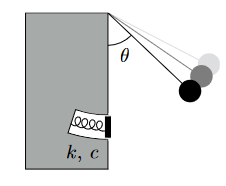
\includegraphics{images/rebound_pendulum_diagram}
        \caption{Diagramm eines Rebound Pendels\cite[6]{flamantSolvingDifferentialEquations2020}}
        \label{fig:rebound_pendulum_diagram}
    \end{figure}
\end{frame}

\begin{frame}{Rebound-Pendel: Netzwerkdaten}
    \begin{table}
        \centering
        \resizebox{\columnwidth}{!}{%
        \begin{tabular}{ l | l }
            \hline
            Netzwerkstruktur & \\
            \hline
            Anzahl der Schichten & $L=10$ \\
            Eingabeschicht & $n^{(0)}=5$ mit $\Phi(x)=\tanh(x)$ \\
            Versteckte Schichten & $n^{(l)}=128$, $l = 1, \dots, L-1$ mit $\Phi(x)=\tanh(x)$ \\
            Ausgabeschicht & $n^{(L)}=2$ mit $\Phi(x)=x$ \\
            \hline
            Hyperparameter und Initialisierungsintervalle & \\
            \hline
            Anfangswertbereiche & $(\theta_0, \varphi_0) \in [0.0, 1.0] \times [-0.2, 0.2]$ \\
            Paramaterbereiche & $(k, c) \in [2.0, 5.0] \times [0.0, 2.0]$ \\
            Zeitraum & $t \in [0, 10]$ \\
            \hline
            Optimierung & \\
            \hline
            Gradientenverfahren & Adam \\
            Gewichtsfunktion & $b(t)=e^{-0.5t}$ \\
            Batch Size & $|B|=10000$ \\
            Epochen & $100000$ \\
            Lernrate & $\eta= 0.0001$ \\
            Gewichtsinitialisierung & Xavier-Initialisierung \\
            \hline
            Statistiken & \\
            \hline
            Trainingrate & 9 Batches/Sekunde  \\
            Trainingszeit & 3.1 Stunden \\
            \hline
        \end{tabular}%
        }
        \label{rebound-pendulum-table}
    \end{table}
\end{frame}

\begin{frame}{Rebound-Pendel: Trajektorien}
    \begin{figure}
        \centering
        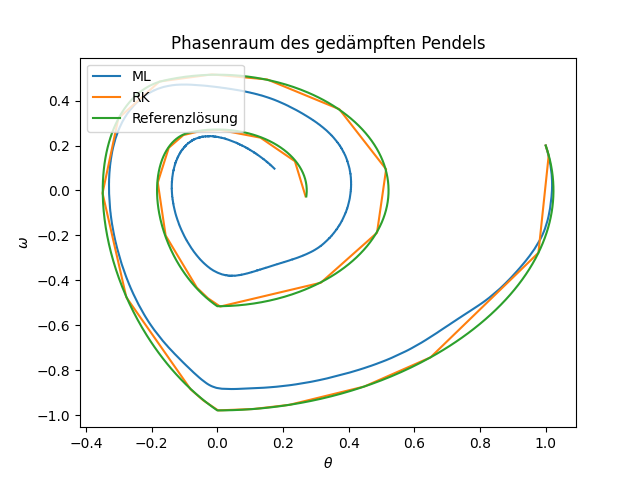
\includegraphics[scale=0.5]{images/Rebound_plots/reboundpendulumtrajectories_}
        \caption{Trajektorie der verschiedenen Lösungen.}
        \label{fig:rebound-trajectories}
    \end{figure}
\end{frame}

\begin{frame}{Rebound-Pendel: $(t,\theta(t))$-Graph}
    \begin{figure}
        \centering
        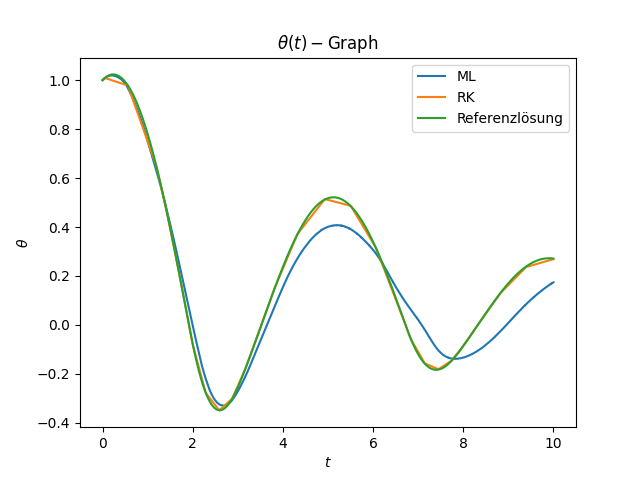
\includegraphics[scale=0.5]{images/Rebound_plots/reboundpendulumtrajectories_in_time_}
        \caption{$(t, \theta(t))$ Graph der berechneten Lösungen.}
        \label{fig:rebound-trajectories-in-time}
    \end{figure}
\end{frame}

\begin{frame}{Rebound-Pendel: Kostenfunktion}
    \begin{figure}
        \centering
        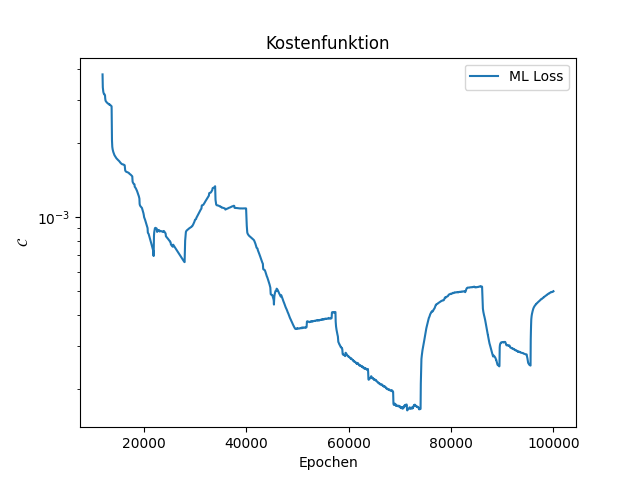
\includegraphics[scale=0.5]{images/Rebound_plots/reboundpendulumavr_loss}
        \caption{Kostenfunktion des neuronalen Netzes bei steigender Epochenanzahl.}
        \label{fig:rebound-loss}
    \end{figure}
\end{frame}


\subsection{Steife Differentialgleichung}

\begin{frame}{Steife Differentialgleichung}
    \begin{itemize}
        \item<1-> Es wird das Anfangswertproblem \eqref{stiff} betrachtet.
        \item<2-> Für die Parameter gilt $c_1=3$, $c_2=4$, $\lambda_1=-100$ und $\lambda_2=-1$.
        \item<3-> Für die relative und globale Toleranz gilt $rtol=10^{-2}$, $atol=10^{-7}$.
    \end{itemize}
\end{frame}

\begin{frame}{Steife Differentialgleichung: Netzwerkdaten}
    \begin{table}
        \renewcommand{\arraystretch}{1.0}
        \centering
        \resizebox{\columnwidth}{!}{%
        \begin{tabular}{ l | l }
            \hline
            Netzwerkstruktur & \\
            \hline
            Anzahl der Schichten & $L=10$ \\
            Eingabeschicht & $n^{(0)}=5$ mit $\Phi(x)=\tanh(x)$ \\
            Versteckte Schichten & $n^{(l)}=32$, $l = 1, \dots, L-1$ mit $\Phi(x)=\tanh(x)$ \\
            Ausgabeschicht & $n^{(L)}=2$ mit $\Phi(x)=x$ \\
            \hline
            Hyperparameter und Initialisierungsintervalle & \\
            \hline
            Anfangswertbereiche &
            $x_{1,0} \in [c_1+c_2 - 0.05, c_1+c_2 + 0.05]$ \\
            & $x_{2,0} \in [c_1-c_2 - 0.05, c_1-c_2 + 0.05]$ \\
            Paramaterbereiche &
            $\lambda_1 \in [\lambda_1 - 0.05, \lambda_1 + 0.05]$ \\
            & $\lambda_2 \in[\lambda_2 - 0.05, \lambda_2 + 0.05]$ \\
            Zeitraum & $t \in [0, 10]$ \\
            \hline
            Optimierung & \\
            \hline
            Gradientenverfahren & Adam \\
%              Gewichtsfunktion & $b(t)=e^{-0.5t}$ \\
            Gewichtsfunktion & $b(t)=1$ \\
            Batch Size & $|B|=10000$ \\
            Epochen & $1000000$ \\
            Lernrate & $\eta= 0.0001$ \\
            Gewichtsinitialisierung & Xavier-Initialisierung \\
            \hline
            Statistiken & \\
            \hline
            Trainingrate & 125 Batches/Sekunde \\
            Trainingszeit & 2.22 Stunden \\
            \hline
        \end{tabular}%
        }
        \label{stiff-table}
    \end{table}
\end{frame}

\begin{frame}{Steife Differentialgleichung: Trajektorien}
    \begin{figure}
        \centering
        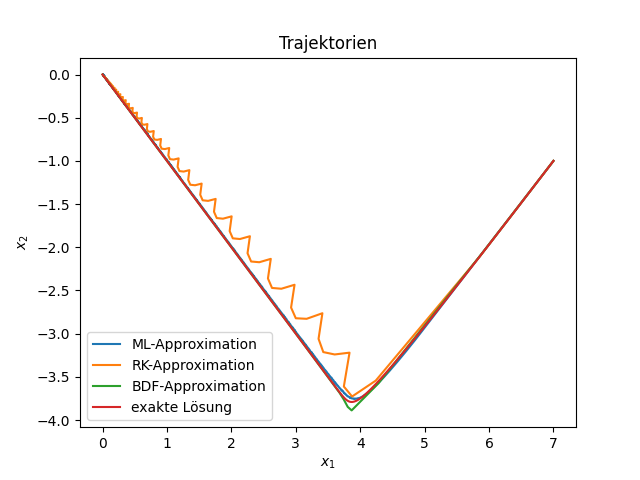
\includegraphics[scale=0.5]{images/Stiff_plots/stifftrajectories_}
        \caption{Trajektorien der verschiedenen Lösungen.}
        \label{fig:stiff-trajectories}
    \end{figure}
\end{frame}

\begin{frame}{Steife Differentialgleichung: Globaler Fehler}
    \begin{figure}
        \centering
        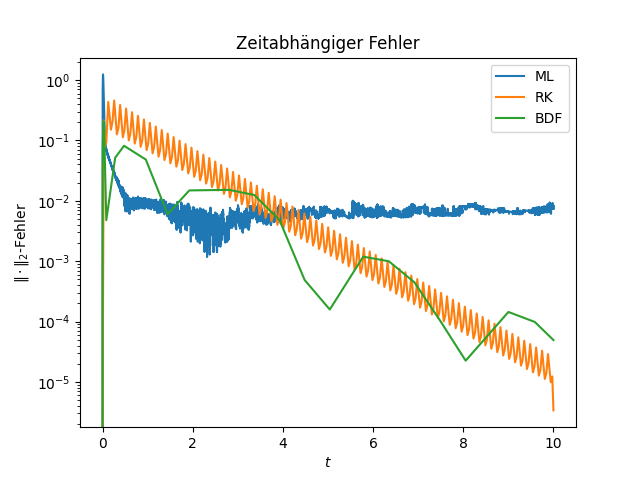
\includegraphics[scale=0.5]{images/Stiff_plots/stiffError_in_time}
        \caption{Globaler Fehler  der jeweiligen Verfahren in Abhängigkeit der Zeit.}
        \label{fig:stiff-error-in-time}
    \end{figure}
\end{frame}

\begin{frame}{Steife Differentialgleichung: Globaler Fehler}
    \begin{figure}
        \centering
        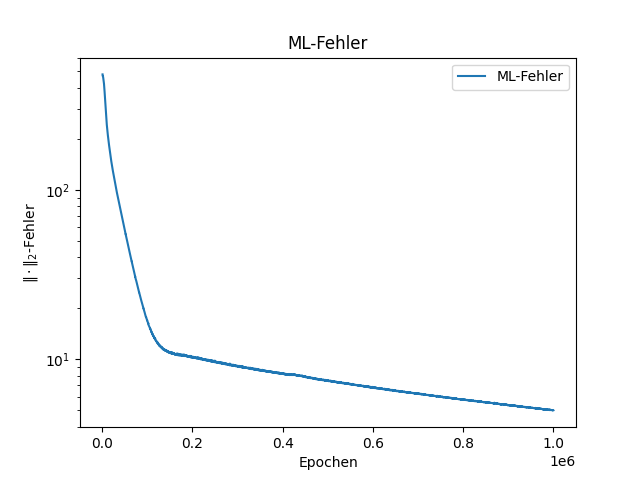
\includegraphics[scale=0.5]{images/Stiff_plots/stiffML_error_}
        \caption{Globaler Fehler für steigende Epochen.}
        \label{fig:stiff-error}
    \end{figure}
\end{frame}

\begin{frame}{Steife Differentialgleichung: Kostenfunktion}
    \begin{figure}
        \centering
        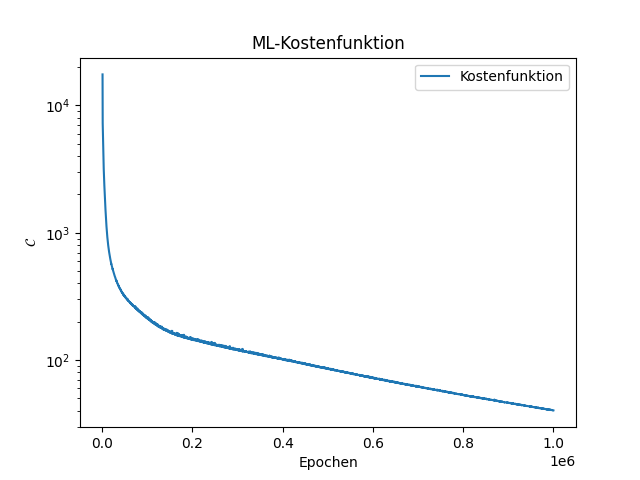
\includegraphics[scale=0.5]{images/Stiff_plots/stiffML_Loss_}
        \caption{Kostenfunktion für steigende Epochen.}
        \label{fig:stiff-loss}
    \end{figure}
\end{frame}


\subsection{Harmonischer Oszillator}

\begin{frame}{Harmonischer Oszillator}
    \begin{itemize}
        \item<1-> Der harmonische Oszillator ist ein Anfangswerproblem erster Ordnung der Form
        \begin{align*}
            &x^{\prime}=v, \qquad v^{\prime}=-\frac{k}{m}x, \\
            &x(0)=0, \quad v(0)=0.
        \end{align*}
        \item<2-> Für die Parameter gilt $m=1$ und $k=1$ für das Runge-Kutta-Verfahren.
        \item<3-> Für die relative und globale Toleranz gilt $rtol=10^{-10}$, $atol=10^{-14}$.
    \end{itemize}
\end{frame}

\begin{frame}{Harmonischer Oszillator: Netzwerkdaten}
    \begin{table}
        \renewcommand{\arraystretch}{1.0}
        \centering
        \resizebox{\columnwidth}{!}{%
        \begin{tabular}{ l | l }
            \hline
            Hyperparameter und Initialisierungsintervalle & \\
            \hline
            Anfangswertbereiche &
            $(x_{0},v_0) \in [-1.0, 1.0] \times [-1.0, 1.0]$ \\
            Paramaterbereiche & $k \in [0.5, 2.0]$ \\
            Zeitraum & $t \in [0, 2\pi]$ \\
            \hline
            Optimierung & \\
            \hline
            Gradientenverfahren & Adam \\
            Gewichtsfunktion & $b(t)=1$ \\
            Batch Size & $|B|=10000$ \\
            Epochen & $100000$ \\
            Lernrate & $0.0001$ \\
            Gewichtsinitialisierung & Xavier-Initialisierung \\
            \hline
        \end{tabular}%
        }
        \caption{Hyperparameter, Initialisierungsintervalle und Optimierungsparameter für den harmonischen Oszillator.}
        \label{stiff-table-data}
    \end{table}
\end{frame}

\begin{frame}{Harmischer Oszillator: Variation 1}
    \begin{table}
        \renewcommand{\arraystretch}{1.0}
        \centering
        \resizebox{\textwidth}{!}{%
        \begin{tabular}{ l | l }
            \hline
            Netzwerk 3 & \\
            \hline
            Anzahl der Schichten & $L=6$ \\
            Eingabeschicht & $n^{(0)}=4$ mit $\Phi(x)=\tanh(x)$ \\
            Versteckte Schichten & $n^{(l)}=16$, $l = 1, \dots, L-1$ mit $\Phi(x)=\tanh(x)$ \\
            Ausgabeschicht & $n^{(L)}=2$ mit $\Phi(x)=x$ \\
            Lernrate & $\eta=0.0001$ \\
            Trainingrate & 195 Batches/Sekunde \\
            Trainingszeit & 0.14 Stunden \\
            \hline
            Netzwerk 4 & \\
            \hline
            Anzahl der Schichten & $L=6$ \\
            Eingabeschicht & $n^{(0)}=4$ mit $\Phi(x)=\tanh(x)$ \\
            Versteckte Schichten & $n^{(l)}=32$, $l = 1, \dots, L-1$ mit $\Phi(x)=\tanh(x)$ \\
            Ausgabeschicht & $n^{(L)}=2$ mit $\Phi(x)=x$ \\
            Lernrate & $\eta=0.0001$ \\
            Trainingrate & 180 Batches/Sekunde \\
            Trainingszeit & 0.15 Stunden \\
            \hline
        \end{tabular}%
        }
    \end{table}
\end{frame}

\begin{frame}{Harmischer Oszillator: Variation 1}
    \begin{table}
        \renewcommand{\arraystretch}{1.0}
        \centering
        \resizebox{\textwidth}{!}{%
            \begin{tabular}{ l | l }
                \hline
                Netzwerk 3 & \\
                \hline
                Anzahl der Schichten & $L=6$ \\
                Eingabeschicht & $n^{(0)}=4$ mit $\Phi(x)=\tanh(x)$ \\
                Versteckte Schichten & $n^{(l)}=16$, $l = 1, \dots, L-1$ mit $\Phi(x)=\tanh(x)$ \\
                Ausgabeschicht & $n^{(L)}=2$ mit $\Phi(x)=x$ \\
                Lernrate & $\eta=0.0001$ \\
                Trainingrate & 195 Batches/Sekunde \\
                Trainingszeit & 0.14 Stunden \\
                \hline
                Netzwerk 4 & \\
                \hline
                Anzahl der Schichten & $L=6$ \\
                Eingabeschicht & $n^{(0)}=4$ mit $\Phi(x)=\tanh(x)$ \\
                Versteckte Schichten & $n^{(l)}=32$, $l = 1, \dots, L-1$ mit $\Phi(x)=\tanh(x)$ \\
                Ausgabeschicht & $n^{(L)}=2$ mit $\Phi(x)=x$ \\
                Lernrate & $\eta=0.0001$ \\
                Trainingrate & 180 Batches/Sekunde \\
                Trainingszeit & 0.15 Stunden \\
                \hline
            \end{tabular}%
        }
    \end{table}
\end{frame}

\begin{frame}{Harmischer Oszillator: Variation 1}
    \begin{figure}
        \centering
        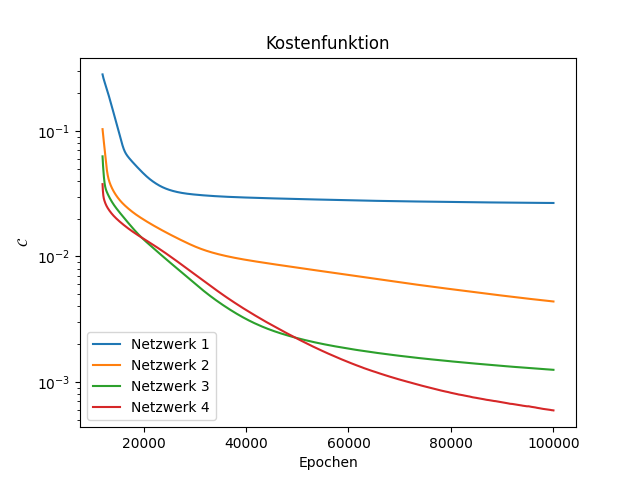
\includegraphics[scale=0.5]{images/harmonicoscillator_plots/harmonicoscillatorML_error__neurons_var_avrloss}
        \caption{Kostenfunktion der verschiedenen neuronalen Netze.}
        \label{fig:harmonic-neurons-variable-loss}
    \end{figure}
\end{frame}

\begin{frame}{Harmischer Oszillator: Variation 1}
    \begin{figure}
        \centering
        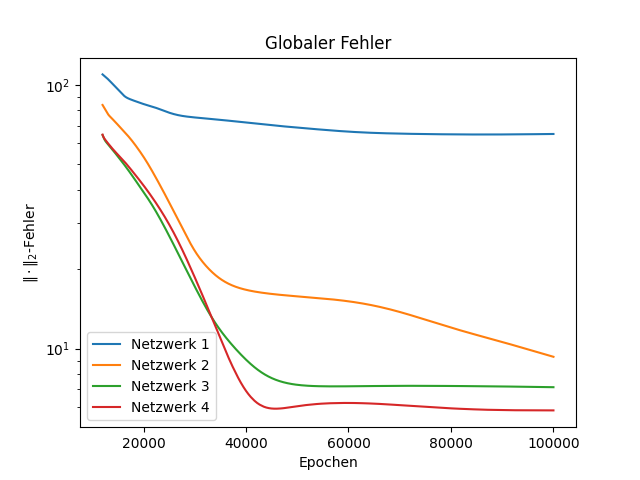
\includegraphics[scale=0.5]{images/harmonicoscillator_plots/harmonicoscillatorML_error__neurons_var_error}
        \caption{Globaler Fehler der verschiedenen neuronalen Netze.}
        \label{fig:harmonic-neurons-variable-error}
    \end{figure}
\end{frame}

\begin{frame}{Harmischer Oszillator: Variation 1}
    \begin{figure}
        \centering
        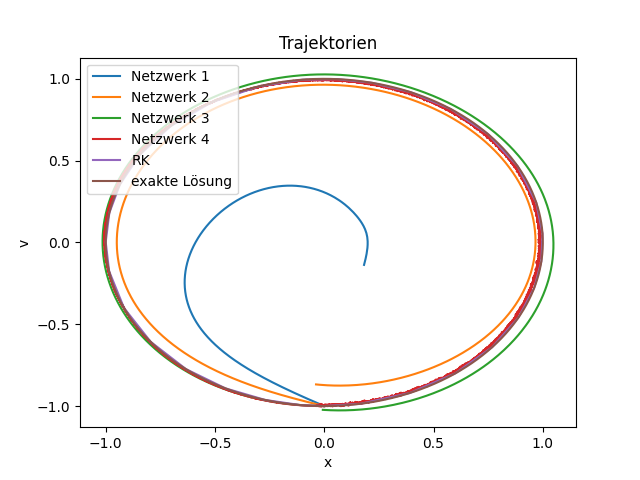
\includegraphics[scale=0.5]{images/harmonicoscillator_plots/harmonicoscillator_neurons_vartrajectories}
        \caption{Trajektorien der von den verschiedenen neuronalen Netzen approximierte Lösung, der Runge-Kutta-Lösung
        und der exakten Lösung.}
        \label{fig:harmonic-neurons-variable-trajectories}
    \end{figure}
\end{frame}

\begin{frame}{Harmischer Oszillator: Variation 1}
    \begin{figure}
        \centering
        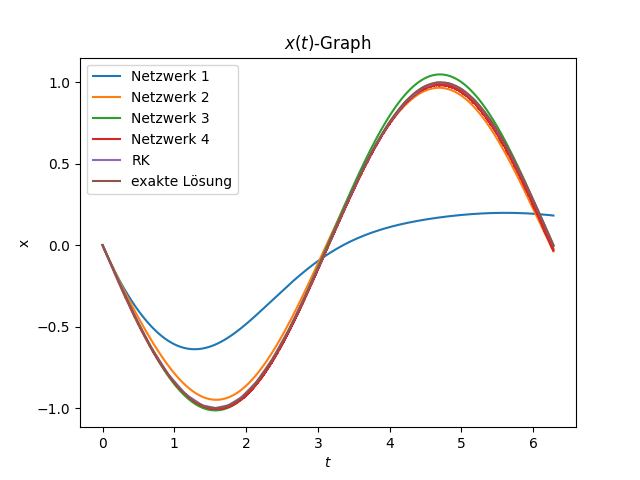
\includegraphics[scale=0.5]{images/harmonicoscillator_plots/harmonicoscillator_neurons_vartrajectories_in_time_}
        \caption{$(t,x(t))$ Graph der Lösungen des Runge-Kutta-Verfahrens, der Approximation der
        Lösungspakete und der exakten Lösung.}
        \label{fig:harmonic-neurons-variable-trajectories-in-time}
    \end{figure}
\end{frame}

\begin{frame}{Harmischer Oszillator: Variation 1}
    \begin{figure}
        \centering
        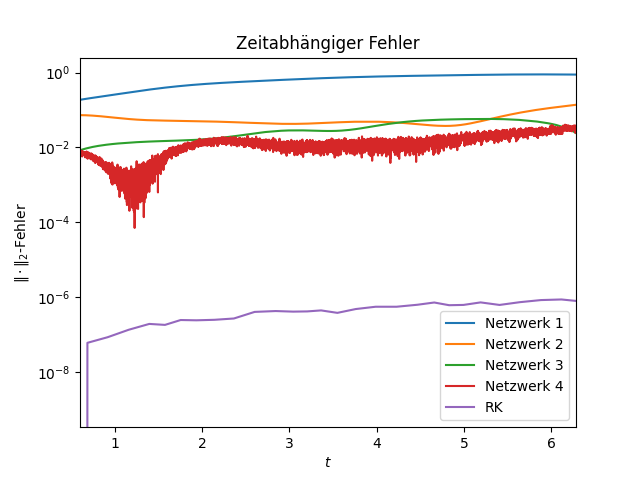
\includegraphics[scale=0.5]{images/harmonicoscillator_plots/harmonicoscillatorError_in_time_neurons_var}
        \caption{Globaler Fehler von Netzwerken $1$ bis $4$ und dem Runge-Kutta-Verfahren in Abhängigkeit der Zeit.}
        \label{fig:harmonic-neurons-variable-error-in-time}
    \end{figure}
\end{frame}

\begin{frame}{Harmonischer Oszillator: Variation 2}
    \begin{table}
        \renewcommand{\arraystretch}{1.0}
        \centering
        \resizebox{\textwidth}{!}{%
        \begin{tabular}{ l | l }
            \hline
            Netzwerk 1 & \\
            \hline
            Anzahl der Schichten & $L=6$ \\
            Eingabeschicht & $n^{(0)}=4$ mit $\Phi(x)=\tanh(x)$ \\
            Versteckte Schichten & $n^{(l)}=32$, $l = 1, \dots, L-1$ mit $\Phi(x)=\tanh(x)$ \\
            Ausgabeschicht & $n^{(L)}=2$ mit $\Phi(x)=x$ \\
            Lernrate & $\eta=0.0001$ \\
            Trainingrate & 185 Batches/Sekunde \\
            Traningszeit & 0.15 Stunden \\
            \hline
            Netzwerk 2 & \\
            \hline
            Anzahl der Schichten & $L=10$ \\
            Eingabeschicht & $n^{(0)}=4$ mit $\Phi(x)=\tanh(x)$ \\
            Versteckte Schichten & $n^{(l)}=32$, $l = 1, \dots, L-1$ mit $\Phi(x)=\tanh(x)$ \\
            Ausgabeschicht & $n^{(L)}=2$ mit $\Phi(x)=x$ \\
            Lernrate & $\eta=0.0001$ \\
            Trainingrate & 129 Batches/Sekunde \\
            Trainingszeit & 0.22 Stunden \\
            \hline
        \end{tabular}%
        }
    \end{table}
\end{frame}

\begin{frame}{Harmonischer Oszillator: Variation 2}
    \begin{table}
        \renewcommand{\arraystretch}{1.0}
        \centering
        \resizebox{\textwidth}{!}{%
        \begin{tabular}{ l | l }
            \hline
            Netzwerk 3 & \\
            \hline
            Anzahl der Schichten & $L=18$ \\
            Eingabeschicht & $n^{(0)}=4$ mit $\Phi(x)=\tanh(x)$ \\
            Versteckte Schichten & $n^{(l)}=32$, $l = 1, \dots, L-1$ mit $\Phi(x)=\tanh(x)$ \\
            Ausgabeschicht & $n^{(L)}=2$ mit $\Phi(x)=x$ \\
            Lernrate & $\eta=0.0001$ \\
            Trainingrate & 76 Batches/Sekunde \\
            Traningszeit & 0.36 Stunden \\
            \hline
        \end{tabular}%
        }
    \end{table}
\end{frame}

\begin{frame}{Harmonischer Oszillator: Variation 2}
    \begin{figure}
        \centering
        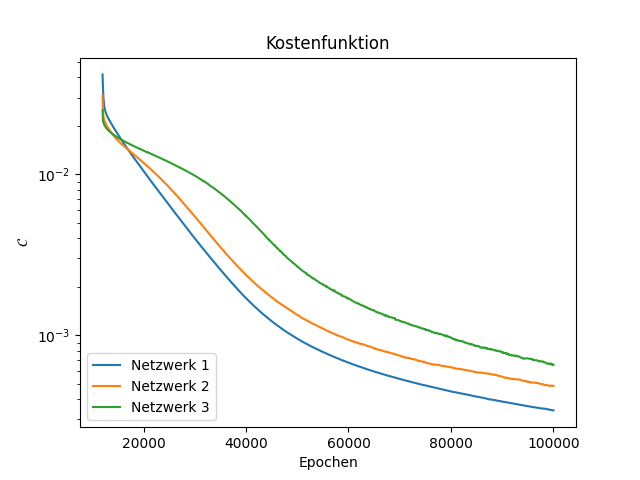
\includegraphics[scale=0.5]{images/harmonicoscillator_plots/harmonicoscillatorML_error__layers_var_avrloss}
        \caption{Kostenfunktion der verschiedenen neuronalen Netze.}
        \label{fig:harmonic-layers-variable-loss}
    \end{figure}
\end{frame}

\begin{frame}{Harmonischer Oszillator: Variation 2}
    \begin{figure}
        \centering
        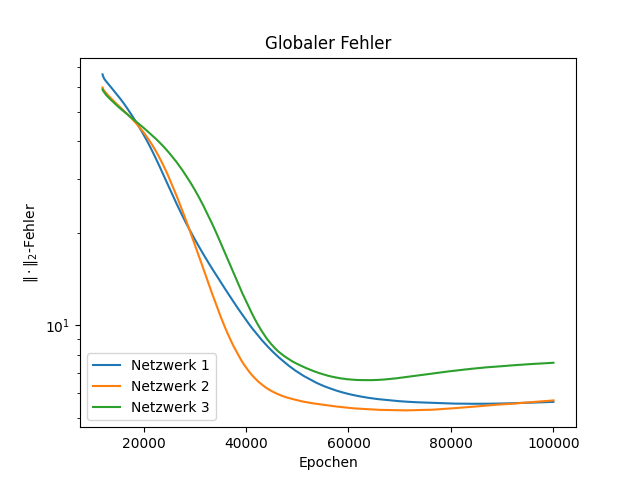
\includegraphics[scale=0.5]{images/harmonicoscillator_plots/harmonicoscillatorML_error__layers_var_error}
        \caption{Globaler Fehler der verschiedenen neuronalen Netze.}
        \label{fig:harmonic-layers-variable-error}
    \end{figure}
\end{frame}

\begin{frame}{Harmonischer Oszillator: Variation 2}
    \begin{figure}
        \centering
        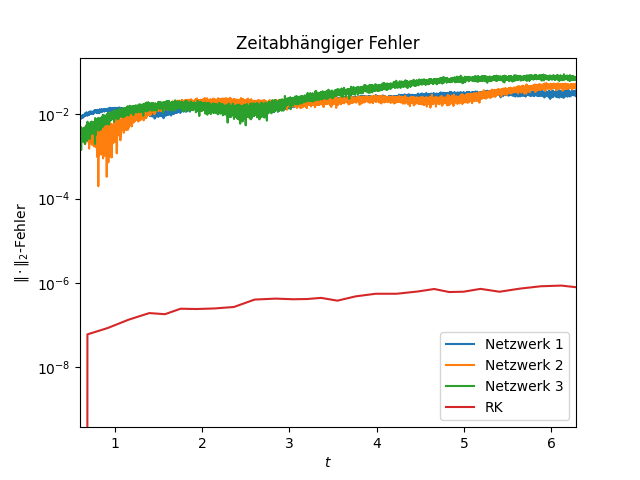
\includegraphics[scale=0.5]{images/harmonicoscillator_plots/harmonicoscillatorError_in_time_layers_var}
        \caption{Globaler Fehler von Netzwerken $1$ bis $3$ und dem Runge-Kutta-Verfahren in Abhängigkeit der Zeit.}
        \label{fig:harmonic-layers-variable-error-in-time}
    \end{figure}
\end{frame}

\begin{frame}{Harmonischer Oszillator: Variation 2}
    \begin{figure}
        \centering
        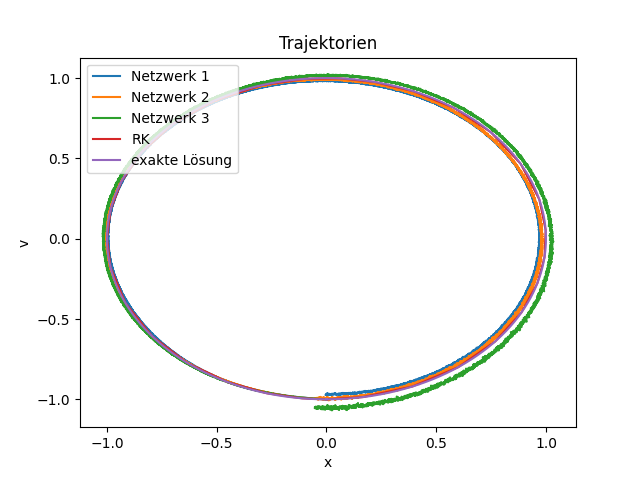
\includegraphics[scale=0.5]{images/harmonicoscillator_plots/harmonicoscillator_layers_vartrajectories}
        \caption{Trajektorien der von den verschiedenen neuronalen Netzen approximierte Lösung, der Runge-Kutta-Lösung
        und der exakten Lösung.}
        \label{fig:harmonic-layers-variable-trajectories}
    \end{figure}
\end{frame}

\begin{frame}{Harmonischer Oszillator: Variation 2}
    \begin{figure}
        \centering
        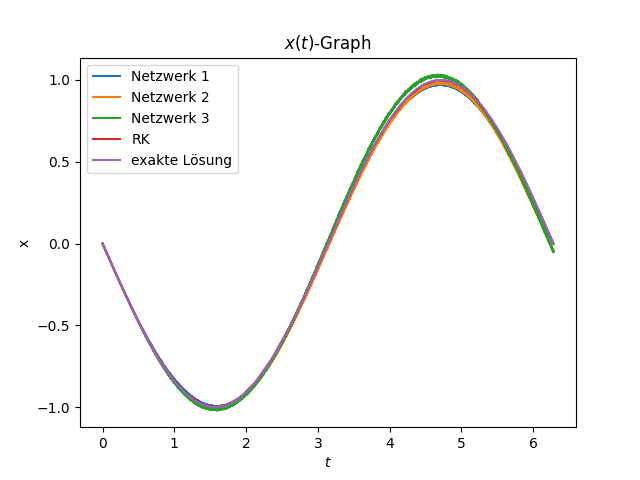
\includegraphics[scale=0.5]{images/harmonicoscillator_plots/harmonicoscillator_layers_vartrajectories_in_time_}
        \caption{$(t,x(t))$-Graph der von den verschiedenen neuronalen Netzen approximierte Lösung, der
        Runge-Kutta-Lösung und der exakten Lösung.}
        \label{fig:harmonic-layers-variable-trajectories-in-time}
    \end{figure}
\end{frame}